\section{Application Implementation}
This section will describe the implementation of the study application, mostly regarding how data was collected, how features were computed as well as how the data was sent to a Firebase instance. 

\subsection{Component Overview}
To provide a high level overview of the different components which make up the study application a component diagram displayed in Figure \ref{fig:app-component-diagram}. The MobilityStudy component in blue is the component responsible for managing the application state but does not do much outside of this since the application state management required is minimal. Had it been a more complex application with many different screens and a state which had to be maintained across these screens (for example a shopping cart in a shopping app) then more logic would lie inside the MobilityStudy component. Instead the Main Screen is spawned from the MobilityStudy component which in turn creates an AppProcessor instance. The AppProcessor instance is responsible for a multitude of tasks, such as asking for permissions, collection location data, and computing features. Storing and loading from the disk is done through the FileManager component which includes location data, Stops, Moves, MobilityContexts and diary answers. This component is also responsible for uploading the stored data to Firebase.

\begin{figure}
    \centering
    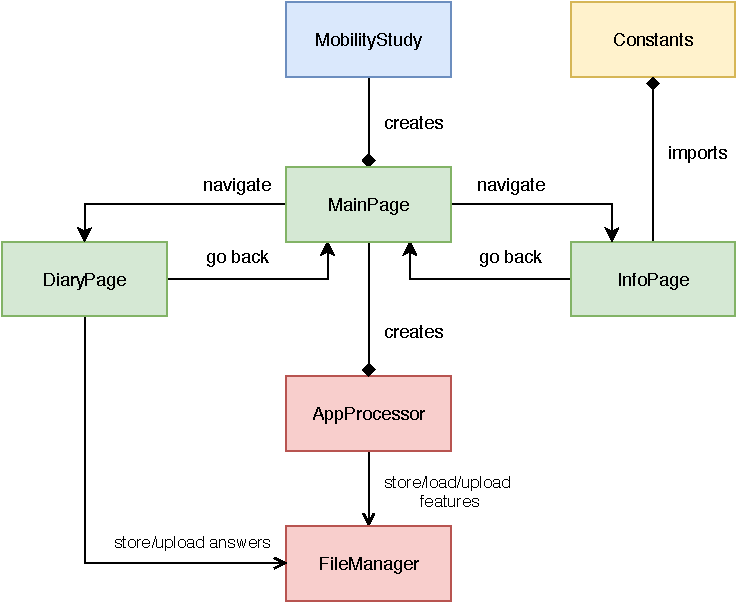
\includegraphics[width=\textwidth]{images/diagrams/app-diagram.pdf}
    \caption{Component diagram for the study application displaying the different building blocks and the interactions between them}
    \label{fig:app-component-diagram}
\end{figure}


\subsection{Location Collection}
The mobile application used the Mobility Features Package by importing it locally using an override as show in Figure \ref{fig:import-package}. As can be seen in the figure, the custom Geolocator plugin previously discussed was also imported in the same manner, since the online version on \url{www.pub.dev} does not allow for background location streaming. 

\begin{figure}
    \centering
    \begin{minted}{yaml}
    dependencies:
      geolocator:
        path: ../geolocator_custom/
      mobility_features:
        path: ../mobility_features/
    \end{minted}
    \caption{Importing the Mobility Features package as well as a custom Geolocator plugin in the \verb|pubspec.yaml| file}
    \label{fig:import-package}
\end{figure}

Next, the location tracking was set up using the Geolocator plugin, in which a stream subscription was initialized which in turn listens for new location data. Each time a new data point comes in, the call-back function \verb|_onData| is called, which handles the data collection. The function uses a buffer and a buffer size; whenever a new datapoint comes in, it is saved to the buffer and if the buffer capacity is reached then all points contained in the buffer are written to the disk, and the buffer is emptied. The lower the buffer size is, the more frequent the location data will be written to the disk.

\begin{figure}
    \centering
    \begin{minted}{dart}
    List<SingleLocationPoint> _pointsBuffer = [];
    static const int BUFFER_SIZE = 100;
    ...
    
    Future _initLocation() async {
        await _geoLocator.isLocationServiceEnabled().then((response) {
          if (response) {
            streamingLocation = true;
            _subscription = _geoLocator.getPositionStream().listen(_onData);
          } else {
            print('Location service not enabled');
          }
        });
    }
    ...
    
    void _onData(Position d) async {
        SingleLocationPoint p =
            SingleLocationPoint(Location(d.latitude, d.longitude), d.timestamp);
        _pointsBuffer.add(p);
    
        // Check if buffer should be saved to disk
        if (_pointsBuffer.length >= BUFFER_SIZE) {
          ...
        }
    }
    \end{minted}
    \caption{Importing the Mobility Features package as well as a custom Geolocator plugin in the \verb|pubspec.yaml| file}
    \label{fig:import-package}
\end{figure}



\subsection{Storing, Loading and Uploading}
Storing and loading SLPs, Stops and Moves work through the serialization API provided by the Mobility Features Package discussed in Chapter \ref{chapter:05}. Concretely a \verb|Serializer<E>| object is created for each type in the AppProcessor class, and are used to store and load their given type \verb|E|. Below is shown an example of this:



\begin{figure}
    \centering
    \begin{minted}{dart}
    Serializer<SingleLocationPoint> _pointSerializer;
    
    ...
    Future<List<SingleLocationPoint>> _loadLocalPoints() async {
        DateTime today = DateTime.now().midnight;
        print('Loading local data points...');
        List<SingleLocationPoint> points = await _pointSerializer.load();
        if (points.isEmpty) {
          return points;
        } else if (points.first.datetime.midnight.isBefore(today)) {
          print('Old location data found, deleting it...');
          points = points.where((p) => p.datetime.midnight == today).toList();
          await _pointSerializer.flush();
          await _pointSerializer.save(points);
        }
        return points;
    }
    \end{minted}
    \caption{The procedure for loading the locally saved SLPs, including filtering out SLPs from previous days}
    \label{fig:points-serialization}
\end{figure}


Whenever new data comes in, the \verb|_onData| callback-method is invoked as previously mention, which collects the new data point in a buffer, which when full is stored to the disk. This is also done by using the Serializer:

\begin{minted}{dart}
if (_pointsBuffer.length >= BUFFER_SIZE) {
    await _pointSerializer.save(_pointsBuffer);
    _pointsBuffer = [];
}
\end{minted}


Saving and loading Stops and Moves is done in a very similar fashion, namely by using separate Serializers. In the case that a MobilityContext is to be computed, the Stops and Moves on disk are loaded with the following source code:

\begin{minted}{dart}
    List<Stop> stops = await _stopSerializer.load();
    List<Move> moves = await _moveSerializer.load();
\end{minted}

After computation, the new-found Stops and Moves are to replace the old ones, which means the Serializers should flush their files, and then store the new data. Given a MobilityContext object \verb|MobilityContext mc| which contains the new Stops and Moves, the parameterless method \verb|flush| is first called, and afterwards the \verb|save| method is called with the new data to be stored.
\begin{minted}{dart}
    await _stopSerializer.flush();
    await _moveSerializer.flush();

    await _stopSerializer.save(mc.stops);
    await _moveSerializer.save(mc.moves);
\end{minted}

\subsection{Computing Features}
Feature calculation was done in an asynchronous manner, in which the work was offloaded to a background thread, rather than running on the main thread. The reason for this is that if the calculation is done on the main thread, then the app will be un-responsive while the computation is being carried out. In the study app there was no real user interface so to speak, but in a real-world application there will be a user interface which cannot be allowed to freeze due to the feature calculation. In FLutter threads are referred to as Isolates which communicate using a SendPort and a ReceivePort. These ports can be used to transfer objects between threads, such that the main thread can ask a background thread to calculate the features, and the background thread will then send back a \textit{MobilityContext} object once finished. To calculate the features, the intermediate features Stops, Moves and Places were calculated first. All this is described by the sequence diagram in Figure \ref{fig:sequence-diagram-mobility-context}, in Chapter \ref{chapter:05}. In figure \ref{fig:feature-comutation-code} source code for achieving this in the flutter app is shown. The \verb|_relay| method works an interface between the \verb|_computeFeaturesAsync| method which runs on the UI thread and the static method \verb|_asyncComputation| which runs on the background thread.


\begin{figure}
    \centering
    \begin{minted}{dart}
    Future<MobilityContext> _computeFeaturesAsync() async {
        // Load from disk
        List<Stop> stops = await _stopSerializer.load();
        List<Move> moves = await _moveSerializer.load();
        List<SingleLocationPoint> points = await _loadLocalPoints();
        
        // Set up background thread
        ReceivePort receivePort = ReceivePort();
        await Isolate.spawn(_asyncComputation, receivePort.sendPort);
        SendPort sendPort = await receivePort.first;
        
        // Off-load computation to background thread, and await
        return await _relay(sendPort, points, stops, moves);
    }
    
    Future _relay(SendPort sp, List<SingleLocationPoint> points, 
                    List<Stop> stops, List<Move> moves) {
    ReceivePort receivePort = ReceivePort();
    sp.send([points, stops, moves, receivePort.sendPort]);
    return receivePort.first;
  }
    \end{minted}
    \caption{The method for querying the Mobility Feature computation on the UI thread}
    \label{fig:feature-comutation-code}
\end{figure}


The \verb|_asyncComputation| method is static which is due to the computation being done in a separate thread than than the main thread. If the objects contained within the AppProcessor instance (i.e. in the main thread) were to change their state while computation was ongoing in the background thread, then the resulting computation would produce an outdated, and or wrong result. To circumvent this, the method that performs the computation relies on parameters instead, i.e. the SLPs, Stops and Moves must be explicitly provided. Concretely, a copy of the objects are created when fed to the static method as parameters. These copies can then have their state modified only inside the static method and not outside which results in the computation being reliable wrt. state management. 

The computation will be discussed bit for bit such a to give the reader a better overview of the implementation:

Firstly the arguments are parsed from the sendport; the arguments come in as an array and are therefore simply extracted via indices.
\begin{minted}{dart}
  static void _asyncComputation(SendPort sendPort) async {
    ReceivePort receivePort = ReceivePort();
    sendPort.send(receivePort.sendPort);
    List args = await receivePort.first;

    /// Extract arguments
    List<SingleLocationPoint> points = args[0];
    List<Stop> stops = args[1];
    List<Move> moves = args[2];
    SendPort replyPort = args[3];
    ...
  }
\end{minted}

Secondly, the date 28 days from today is calculated and from this date a filtering process for the loaded Stops and Moves is performed. This process removes all the loaded Stops and Moves which are today, or older than four weeks from today. The reason for removing data from today is that it must be recalculated using all the data points from today, in order to be precise. Secondly data older than 28 days is discarded since it is no longer relevant, the concrete reasons are discussed in Chapter \ref{chapter:03}.
\begin{minted}{dart}
    DateTime today = DateTime.now().midnight;
    DataPreprocessor preprocessor = DataPreprocessor(today);
    DateTime fourWeeksAgo = today.subtract(Duration(days: 28));

    /// Filter out stored stops and moves which were computed today,
    /// as well as stops older than 4 weeks
    List<Stop> stopsOld = stops.isEmpty
        ? stops
        : stops
            .where((s) =>
                s.arrival.midnight != today.midnight &&
                fourWeeksAgo.leq(s.arrival.midnight))
            .toList();

    List<Move> movesOld = moves.isEmpty
        ? moves
        : moves
            .where((m) =>
                m.stopFrom.arrival.midnight != today.midnight &&
                fourWeeksAgo.leq(m.stopFrom.arrival.midnight))
            .toList();
\end{minted}

Thirdly, today's data points are used to find the most updated set of Stops and Moves for today, which are then concatenated with the old stops and moves. From this set of intermediate features covering the last 28 days the corresponding Places for the period can now be found.

\begin{minted}{dart}
    /// Calculate stops and moves from today
    List<Stop> stopsToday = preprocessor.findStops(points, filter: false);
    List<Move> movesToday = preprocessor.findMoves(points, stopsToday, filter: false);

    /// Concatenate old and new, and compute places
    List<Stop> stopsAll = stopsOld + stopsToday;
    List<Move> movesAll = movesOld + movesToday;
    List<Place> placesAll = preprocessor.findPlaces(stopsAll);
\end{minted}

Lastly, the MobilityContex is computed from the intermediate features from the whole period
\begin{minted}{dart}
    /// Compute features
    MobilityContext mobilityContext = MobilityContext(today, stopsAll, placesAll, movesAll);
    replyPort.send(mobilityContext);
\end{minted}